%%%%%%%%%%%%%%%%%%%%%%%%%%%%%%%%%%%%%%%%%%%%%%%%%%%%%%%%%%%%%%%%%%%%%%%%%%%%%%%%%%%%%%
% To make formatting easy tell LaTeX what kind of document you want to write
% by changing the according {} to {#1}
%%%%%%%%%%%%%%%%%%%%%%%%%%%%%%%%%%%%%%%%%%%%%%%%%%%%%%%%%%%%%%%%%%%%%%%%%%%%%%%%%%%%%%


%%%%%%%%%%%%%%%%%%%%%%%%%%%%%%%%%%%%%%%%%%%%%%%%%%%%%%%%%%%%%%%%%%%%%%%%%%%%%%%%%%%%%%
% Which language do you want to write in
%%%%%%%%%%%%%%%%%%%%%%%%%%%%%%%%%%%%%%%%%%%%%%%%%%%%%%%%%%%%%%%%%%%%%%%%%%%%%%%%%%%%%%
%English
\newcommand{\EN}[1]{#1}
%German
\newcommand{\DE}[1]{}

%%%%%%%%%%%%%%%%%%%%%%%%%%%%%%%%%%%%%%%%%%%%%%%%%%%%%%%%%%%%%%%%%%%%%%%%%%%%%%%%%%%%%%
% For print single or double page?
%%%%%%%%%%%%%%%%%%%%%%%%%%%%%%%%%%%%%%%%%%%%%%%%%%%%%%%%%%%%%%%%%%%%%%%%%%%%%%%%%%%%%%
\newcommand{\single}[1]{#1}
\newcommand{\double}[1]{}

%%%%%%%%%%%%%%%%%%%%%%%%%%%%%%%%%%%%%%%%%%%%%%%%%%%%%%%%%%%%%%%%%%%%%%%%%%%%%%%%%%%%%%
% Now this is followed by a lot of page and command definitions. For the beginning you 
% should be able to continue where you find the next comment section like this one.
% However, you might want to take a look a the definitions sometime to be able to use 
% them. Of course you can also add the defintions you needed yourself.
%%%%%%%%%%%%%%%%%%%%%%%%%%%%%%%%%%%%%%%%%%%%%%%%%%%%%%%%%%%%%%%%%%%%%%%%%%%%%%%%%%%%%%

\single{\documentclass[12pt,a4paper,oneside,english]{book}}
\double{\documentclass[12pt,a4paper,twoside,english]{book}}

\usepackage[english]{babel}
%\usepackage[draft,breaklinks=true,colorlinks=false,dvips,bookmarks,pdffitwindow,pdfcenterwindow=true,pdfstartview=Fit]{hyperref}
%\usepackage[breaklinks=true,colorlinks=false,dvips,bookmarks,pdffitwindow,pdfcenterwindow=true,pdfstartview=Fit]{hyperref}
\usepackage{graphicx}
\usepackage{xcolor}
\usepackage{caption}
\usepackage{subcaption}
\usepackage{setspace}
\usepackage{cite}
\usepackage{float,times} 
\usepackage[utf8x]{inputenc}
\usepackage[T1]{fontenc}
\usepackage{amsmath,amsthm,latexsym}
\usepackage[dvips]{epsfig}
%\usepackage{subfigure}
\usepackage{rotating}
\usepackage{afterpage}
\usepackage{multirow}
\usepackage{array}

\usepackage[outputdir=obj]{minted}
\usepackage{newfloat}
\usepackage{xspace}
%! put the new-command after the inputenc package use, so 'ü' will not be shown as abomination ASCII -TF
	
%%%%%%%%%%%%
%%% MINTED
%%%%%%%%%%%%

\DeclareFloatingEnvironment[
  fileext=loc,
  listname=List of Listings,
  name=Listing,
  placement=htp,
]{codefloat}

\newenvironment{vhdl}[2][]
 {\codefloat[htb]
  \if\relax\detokenize{#1}\relax\else\caption{#1}\fi
  \if\relax\detokenize{#2}\relax\else\label{#2}\fi 
  \minted[%linenos,
          %numbersep=5pt,
          tabsize=3,
          frame=lines,
          framesep=2mm,
          fontsize=\footnotesize]
         {vhdl}}
 {\endminted
 \endcodefloat}
\newenvironment{asm}[2][]
 {\codefloat[htb]
  \if\relax\detokenize{#1}\relax\else\caption{#1}\fi
  \if\relax\detokenize{#2}\relax\else\label{#2}\fi 
  \minted[%linenos,
          %numbersep=5pt,
          tabsize=3,
          frame=lines,
          framesep=2mm,
          fontsize=\footnotesize]
         {c}}
 {\endminted
 \endcodefloat}

%%%%%%%%%%%%
%%% COMMENTS AND TODO-MARKERS
%%%%%%%%%%%%

% \newcommand{\comment}[3]{\marginpar{\textcolor{#2}{Comment: #1}}\textcolor{#2}{\textit{[#1: #3]}}}
% \newcommand{\TF}[1]{\comment{TF}{orange}{#1}}
% \newcommand{\LS}[1]{\comment{LS}{blue}{#1}}
% 
% \newcommand{\qn}{\todo{qn!}}
% \newcommand{\sectodo}{\todo{Still todo.}}
% \newcommand{\seccheck}{\marginpar{\textcolor{orange}{reread}}}
% \newcommand{\secthomas}{\marginpar{\textcolor{green}{thomas}}}
% \newcommand{\secdone}{\marginpar{\textcolor{gray}{done}}}
% %\newcommand{\todo}[1]{\pagecolor{red!10}\afterpage{\nopagecolor}\textcolor{red}{\textit{[#1]}}\marginpar{\textcolor{red}{\textbf{TODO}}}}
% \newcommand{\todo}[1]{\textcolor{red}{\textit{[#1]}}\marginpar{\textcolor{red}{\textbf{TODO}}}}
% 
% 
% %%% BLANK COMMANDS FOR PUBLISHING
% \newcommand{\publish}[1]{}
% \renewcommand{\publish}[1]{#1} % TODO: uncomment this line before printing!
% 
% \publish{\renewcommand{\comment}[3]{}}
% \publish{\renewcommand{\TF}[1]{}}
% \publish{\renewcommand{\LS}[1]{}}
% \publish{\renewcommand{\qn}{}}
% \publish{\renewcommand{\sectodo}{}}
% \publish{\renewcommand{\seccheck}{}}
% \publish{\renewcommand{\secthomas}{}}
% \publish{\renewcommand{\secdone}{}}
% \publish{\renewcommand{\todo}[1]{}}

\newcommand{\comment}[3]{\marginpar{\textcolor{#2}{Comment: #1}}\textcolor{#2}{\textit{[#1: #3]}}}
\newcommand{\TF}[1]{\comment{TF}{red}{#1}}
\newcommand{\TS}[1]{\comment{TS}{blue}{#1}}
\newcommand{\FP}[1]{\comment{TS}{orange}{#1}}

%%%%%%%%%%%%
%%% LOGIC OPERATORS
%%%%%%%%%%%%

\newcommand{\logicxor}{\texttt{XOR}\xspace}
\newcommand{\logicor}{$||$\xspace}%TODO: does not show up as OR
\newcommand{\logicand}{\&\xspace}

%%%%%%%%%%%%
%%% STUFF
%%%%%%%%%%%%

\newcommand{\mem}[1]{*#1\xspace}
\newcommand{\x}{--\xspace}

%%%%%%%%%%%%
%%% NAMES
%%%%%%%%%%%%

\newcommand{\procname}{\textsl{LT16x32}\xspace}

%%%%%%%%%%%%
%%% FORMAT SHORTCUTS
%%%%%%%%%%%%

\newcommand{\floatplace}{[ht]}

\newcommand{\tc}[1]{\textbf{#1}}

\newcommand{\hex}[1]{#1}
\newcommand{\bits}[1]{#1}

\newcommand{\filename}[1]{{\small\texttt{#1}}}
\newcommand{\command}[1]{{\small\texttt{#1}}}
\newcommand{\inlinevhdl}[1]{{\small\texttt{#1}}} %TODO with syntax highlighting and check for $\_$
\newcommand{\inlinec}[1]{{\small\texttt{#1}}} %TODO with syntax highlighting and check for $\_$
\newcommand{\inlineasm}[1]{{\small\texttt{#1}}} %TODO with syntax highlighting and check for $\_$

\newcommand{\instruction}[7]{
\subsubsection{#1}
\label{instr_#2}
\begin{description}
\nolistskip
\item[Opcode:] \texttt{#3}
\item[Assembler:] \inlineasm{#4}
\item[Operation:] #5
\item[C-Equivalent:] \inlinec{#6}
\item[Status Register:] #7
\end{description}
}


%%%%%%%%%%%%
%%% TEX WORKAROUNDS
%%%%%%%%%%%%
\newcommand{\nolistskip}{\itemsep-3pt}

\newcommand{\DocuTitle}{Documentation of the LT16x32 System-on-Chip}

% format page layout.
\setlength{\topmargin}{0cm}
\setlength{\textwidth}{15cm}
\setlength{\textheight}{22cm}
\setlength{\oddsidemargin}{1cm}
\setlength{\evensidemargin}{0cm}

\setlength{\headheight}{15pt}
% \setlength{\voffset}{-0cm}
% \setlength{\topmargin}{0cm}
% \setlength{\headheight}{0.54cm}
% \setlength{\textheight}{23cm}
% % \setlength{\headsep}{1.5cm}
% %\setlength{\hoffset}{-2.54cm}
% \setlength{\hoffset}{0cm}
% \setlength{\oddsidemargin}{0.46cm}
% \setlength{\evensidemargin}{0.46cm}
% \setlength{\textwidth}{15cm}
% \setlength{\marginparsep}{0cm}
% \setlength{\marginparwidth}{1.54cm}

\setcounter{secnumdepth}{3}


% \setlength{\footskip}{1cm}
% \setlength{\parindent}{0cm}
% \setlength{\parskip}{1em}

\usepackage{fancyhdr}
\pagestyle{fancy}
\fancyhead{} % clear all header fields
%\fancyhead[LO, RE]{\slshape \nouppercase{\leftmark}} % chapter titles
%\fancyhead[LE, RO]{\slshape \nouppercase{\leftmark}\\\nouppercase{\rightmark}} % section titles
\double{\fancyhead[LE]{\slshape \nouppercase{\leftmark}}} % chapter titles
\fancyhead[RO]{\slshape \nouppercase{\rightmark}} % section titles
\fancyfoot{} % clear all footer fields
\fancyfoot[C]{\thepage}


\usepackage[%dvips,
	colorlinks=false,
	bookmarks,
	pdffitwindow,
	pdfcenterwindow=true,
	pdfstartview=Fitpdftex,
	pdfauthor={Lasse Schnepel, Thomas Fehmel},
	pdftitle={\DocuTitle},
	pdfsubject={LT16x32 Documentation}, % one sentence summery
	pdfkeywords={Processor,Firmware-based Verification,Architecture design}, %comma-seperated keywords
	pdfproducer={Latex with hyperref},
	pdfcreator={}]{hyperref}

\begin{document}

% \EN{\selectlanguage{english}}
% \DE{\selectlanguage{german}}


%%%%%%%%%%%%%%%%%%%%%%%%%%%%%%%%%%%%%%%%%%%%%%%%%%%%%%%%%%%%%%%%%%%%%%
% Here you have to start editing
%%%%%%%%%%%%%%%%%%%%%%%%%%%%%%%%%%%%%%%%%%%%%%%%%%%%%%%%%%%%%%%%%%%%%%
\title{\DocuTitle}
\author{Lasse Schnepel, Thomas Fehmel}
\date{2015}
\pagenumbering{arabic} 
\hyphenation{Bit-ebenen Gateprop Bit-ebene Fanin Boole-sche
  Partial-produkt-generator
  Code-inspektion
  Verifika-tions-ablauf
  IPC-Verifika-tions-ablauf
  Abhangig-keiten
}


%%%%%%%%%%%%%%%%%%%%%%%%%%%%%%%%%%%%%%%%%%%%%%%%%%%%%%%%%%%%%%%%%%%%%%%%
% title page
%%%%%%%%%%%%%%%%%%%%%%%%%%%%%%%%%%%%%%%%%%%%%%%%%%%%%%%%%%%%%%%%%%%%%%%%
\frontmatter
\maketitle
\tableofcontents

\mainmatter

%%%%%%%%%%%%%%%%%%%%%%%%%%%%%%%%%%%%%%%%%%%%%%%%%%%%%%%%%%%%%%%%%%%%%%%
% Now this is followed by your chapters
% this usually starts with introduction and Fundamentals and then 
% continues with whatever you need or did
%%%%%%%%%%%%%%%%%%%%%%%%%%%%%%%%%%%%%%%%%%%%%%%%%%%%%%%%%%%%%%%%%%%%%%%

\chapter{Scope of Delivery}
\section{Products}
Containing in the ESyLab-SoC are the the processor core \procname, 
a configurable Wishbone bus interconnect module, 
a minimal interrupt controller and peripheral devices.

An instruction memory is also supplied.
It reads a file with machine code during elaboration, 
so the SoC can both be simulated and synthesized.
The assembler to produce that machine code is also supplied in source.

\section{HowTo: Build Products}
\label{sec:scope_build}
The products are delivered as HDL source code. 
This allows adaptation to any platform, for which the needed tools are available (see sections below).

\subsection{Processor}
The processor is delivered as a set of VHDL files, including one top entity (processor in \filename{processor.vhd}) which can be used in any VHDL synthesis tool.
For simulation, the entity \inlinevhdl{core\_tb} (in \filename{core\_tb.vhd}) can be used. Both architectures instantiate the core, a memory controller and a interrupt controller.
The filename of the used program can be set in these files in the generic map of the memory controller instantiation (see Listing \ref{lst:memory_file}).
Here, also the memory size can be determined (as number of stored words). For details on the memory controller see Section \ref{sec:memoryctrl}.

\begin{vhdl}[Generic Map Extract of Memory Controller]{lst:memory_file}
memory_inst : component memory
	generic map(filename     => "../programs/test.ram",
		        size         => 32,
		        [...]
		        )
\end{vhdl}

The processor is wrapped in another module,
which implements the Wishbone bus-interface for the data memory interface of the processor.

\subsection{Bus Interconnect}
The bus interconnect system is configureable to any number of slave and master modules,
the appropriate configuration values (see Listing~\ref{lst:wishbone_config}) can be found in the file \verb=lib/wishbone.vhd=.
\begin{vhdl}[Wishbone interconnect configuration]{lst:wishbone_config}
...
constant NWBMST:	integer	:=4; 
	--Number of Wishbone master connectors on the Interconnect
constant NWBSLV:	integer :=16; 
	--Number of Wishbone slave connectors on the Interconnect
...
\end{vhdl}
All connections can be masked during its instantiation,
using the slave and master mask vectors (see Listing~\ref{lst:wishbone_mask_config}).
They are declared in the top level architecture and are used during instantiation of the interconnection component.
\begin{vhdl}[Wishbone interconnect configuration]{lst:wishbone_mask_config}
...
	constant slv_mask_vector : std_logic_vector(0 to NWBSLV-1) := b"1110_0000_0000_0000";
	constant mst_mask_vector : std_logic_vector(0 to NWBMST-1) := b"1000";
...
\end{vhdl}
The component handles synchronous Wishbone cycle termination.

\subsection{Assembler}
For building the assembler the GNU tools \filename{gcc}, \filename{make}, \filename{bison} and \filename{flex} are needed. With these tools installed, the \filename{make} script can be used to generate an executable called \filename{asm}:
\begin{verbatim}
	($SOCROOT)/assembler/$ make all
\end{verbatim}

It is recommended to either copy or dynamically link the assembler executable in a directory in your \verb=$PATH= or  directly referenced by in your build tool chain.

\chapter{SoC Architecture}\label{chap:socarch}
The supplied ESyLab-SoC plattform is implemented by the \verb=top.vhd=,
which can be found in the \verb=<project root>/soc/top= directory.
Its structure is illustrated by Figure~\ref{fig:socoverview}.
\begin{figure}[htb]
	\centering
	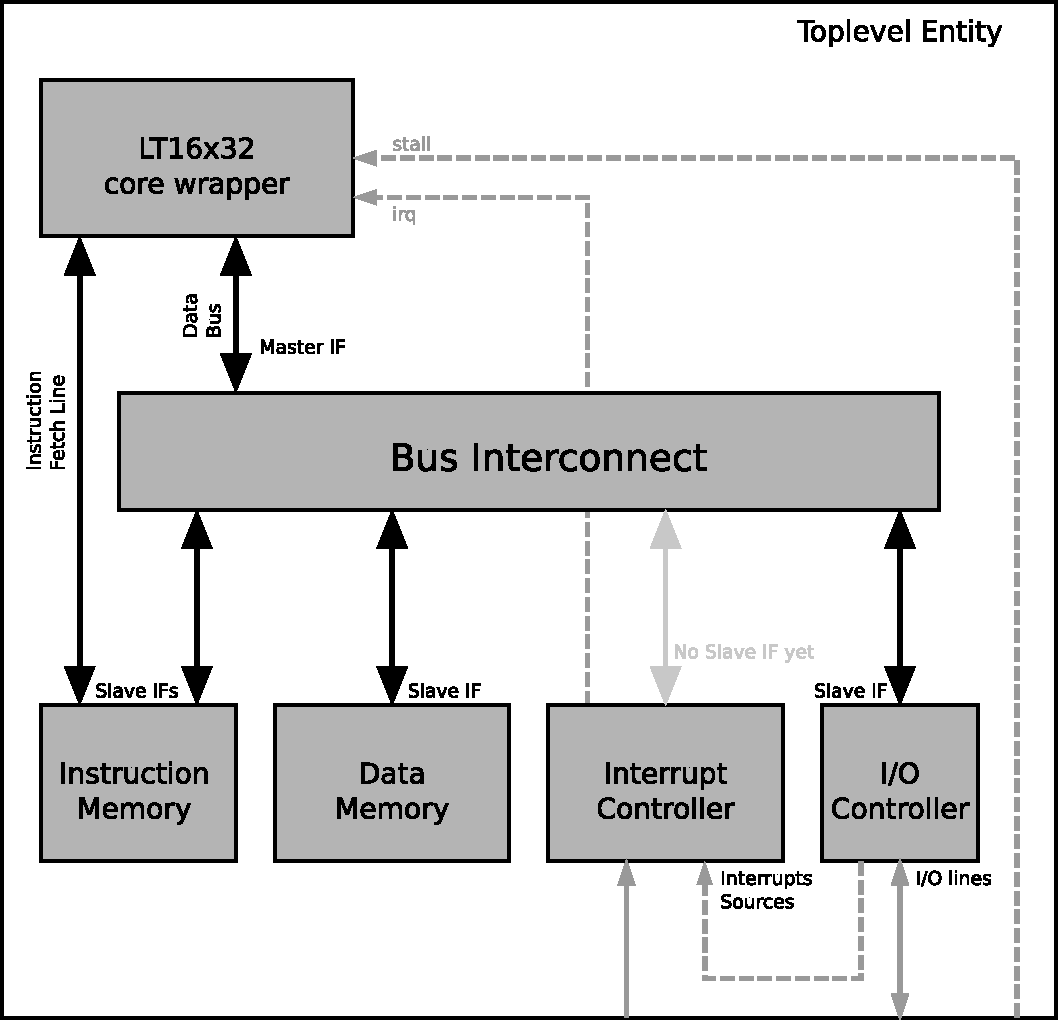
\includegraphics[scale=0.55]{./figures/soc_overview.pdf}
	\caption{Block diagram of the ESyLab-SoC}
	\label{fig:socoverview}
\end{figure}

The interface of the minimal top level entity of the \procname system is shown in Listing~\ref{lst:top_interface}.
\begin{vhdl}[Top Level Entity]{lst:top_interface}
entity lt16soc_top is
generic(
  programfilename : string := "programs/program.ram"
);
port(
  clk		: in  std_logic;
  rst		: in std_logic;
  
  led		: out std_logic_vector(7 downto 0)
);
end entity lt16soc_top;
\end{vhdl}

The inputs \inlinevhdl{clk}, which denote the clock input, and \inlinevhdl{rst}, which is the active high reset, are system-wide signals. 
The minimal system features only one output signal, which is \inlinevhdl{led}.
This signal should be connected to a set of leds and is connected to a generic I/O-controller on the bus.

The individual components of the minimal system are described in the following sections.

\section{Interconnect}
\label{chap:socarch:interconnect}
The system utilizes a synchronous Wishbone bus.
To ease integration of new bus components, a Wishbone bus interconnect component is provided.
The interconnect module currently implements only the synchronous Whisbone protocol.
Its interface is given in Listing~\ref{lst:wb_interconnect_interface}.

\begin{vhdl}[Top Level Entity]{lst:wb_interconnect_interface}
entity wb_intercon is
generic(
  slv_mask_vector : std_logic_vector(0 to NWBSLV-1) := 0;
  mst_mask_vector : std_logic_vector(0 to NWBMST-1) := 0
);
port(
  clk  : in  std_logic;
  rst  : in  std_logic;
  msti : out wb_mst_in_vector;
  msto : in  wb_mst_out_vector;
  slvi : out wb_slv_in_vector;
  slvo : in  wb_slv_out_vector 
);
\end{vhdl}
The system is configured to a certain maximum number of slave and master modules as \inlinevhdl{NWBSLV} and \inlinevhdl{NWBMST} respectively. 
The configuration can be found in \verb=config.vhd=.

These constants are used to define a the length of two generic parameters of the module,
the mask vectors \verb=slv_mask_vector= and \verb=mst_mask_vector=, 
and also define how many elements the input and output arrays have.
As for the mask vectors, as indicated in the \verb=wishbone.vhd= file.
The mask vectors are used to indicate to the interconnect if a module should be connected to the input/output port indicated by the bit position in the mask vector.
A '1' at a position in the mask vector indicates that at the respective position in the the input/output arrays, 
a module should be connected.
A '0' at a position in the mask vector will facilitate that the control logic for that position in the respective input/output array is omitted.

The inputs \inlinevhdl{clk} and \inlinevhdl{rst} are currently not used, but might be in the future when synchronous wishbone transfer is implemented.

The wishbone bus signals are separated in arrays of master and slave signals.
Array of master signals is in the output \inlinevhdl{msti}, which are the inputs to the connected masters, and the input \inlinevhdl{msto}, which are the outputs of the connected master.
Analogously, \inlinevhdl{slvi} and \inlinevhdl{slvo} follow the same principle for the connected slave modules.

\subsection{Integration of new components}
To instantiate a new component in the system, 
a few steps must be undertaken.

\paragraph{The component declaration}%
should not be put in the top level module, 
but in the appropriate package.
This makes the top level module more readable.

\paragraph{The component instantiation}%
in the top level module must be connected to the bus interconnect system.
To do this, the port map must connect its inputs and outputs of its bus interface to a free element of the \verb=slvi= and \verb=slvo= array signals in the top level architecture.
Any element in that vector must obviously only be assigned once.

To select to which of those signals you should connect,
consult the file \verb=soc/lib/config.vhd=.
A number of of slave index constants like shown in Listing~\ref{lst:config_constants} are defined there.
Add your own by adding one to the last defined constant,
then use the defined constant to select the element of the bus slave signal arrays, as illustrated in Listing.~\ref{lst:slave_port_assignment}.

\begin{vhdl}[Slave bus indexes]{lst:config_constants}
-- >> Slave index  <<
constant CFG_MEM : integer := 0; 
constant CFG_LED : integer := CFG_MEM+1;
constant CFG_DMEM : integer := CFG_LED+1;
...
\end{vhdl}
\begin{vhdl}[Slave bus connection]{lst:slave_port_assignment}
... port map( ...
wslvi		=> slvi(CFG_FOO),
wslvo		=> slvo(CFG_FOO)
...
\end{vhdl}

\paragraph{The slave masking vector}%
is a constant which configures the interconnect system to only consider certain slave bus interface elements.
A slave mask vector \verb=slv_mask_vector= is defined in the top level architecture, see Listing~\ref{lst:slave_mask}.
To enable any connection on the interconnect,
the bit in the slave mask vector must be set to '1' at the same position as the targeted elements in the slave connector arrays.

Setting any bit in the slave mask vector to '0' will disable the corresponding connection to the interconnection in the way that the logic to evaluate the inputs is not generated.

\begin{vhdl}[Slave bus indexes]{lst:slave_mask}
architecture RTL of lt16soc_top is
...
constant slv_mask_vector : std_logic_vector(0 to NWBSLV-1) := b"1110_0000_0000_0000";
...
\end{vhdl}

\section{Processor Core Wrapper}
The processor core has a data and instruction memory interface, as per standard Harvard architecture.
The instruction memory interface is unchanged, but the data memory interface is wrapped in a piece of control logic translating the processor interface to wishbone signals and takes care of timing.

\section{Instruction memory}
The instruction memory component is configurable to load a file into its memory during elaboration.
The loaded file needs to contain legal values of the type std\_logic\_vector with a length of 32 characters per line.
If the content of the file is illegal, an error in the elaboration tool will likely occur.

It has two interfaces, one for instruction read access by the processor, one for a read and write access by the Wishbone bus.
The Wishbone interface takes priority over the instruction read.
The whole range of the memory can be written, so care should be exercised when writing to the instruction memory, 
so code or 'constants' are not unintentionally overwritten.

\chapter{Processor Architecture}
\section{Block Diagram}
A simplified block diagram of the \procname can be found in Figure \ref{fig:blockdiagram_core}.
A diagram of the datapath can be found in Figure \ref{fig:blockdiagram_dp}

\begin{figure}[htb]
	\centering
	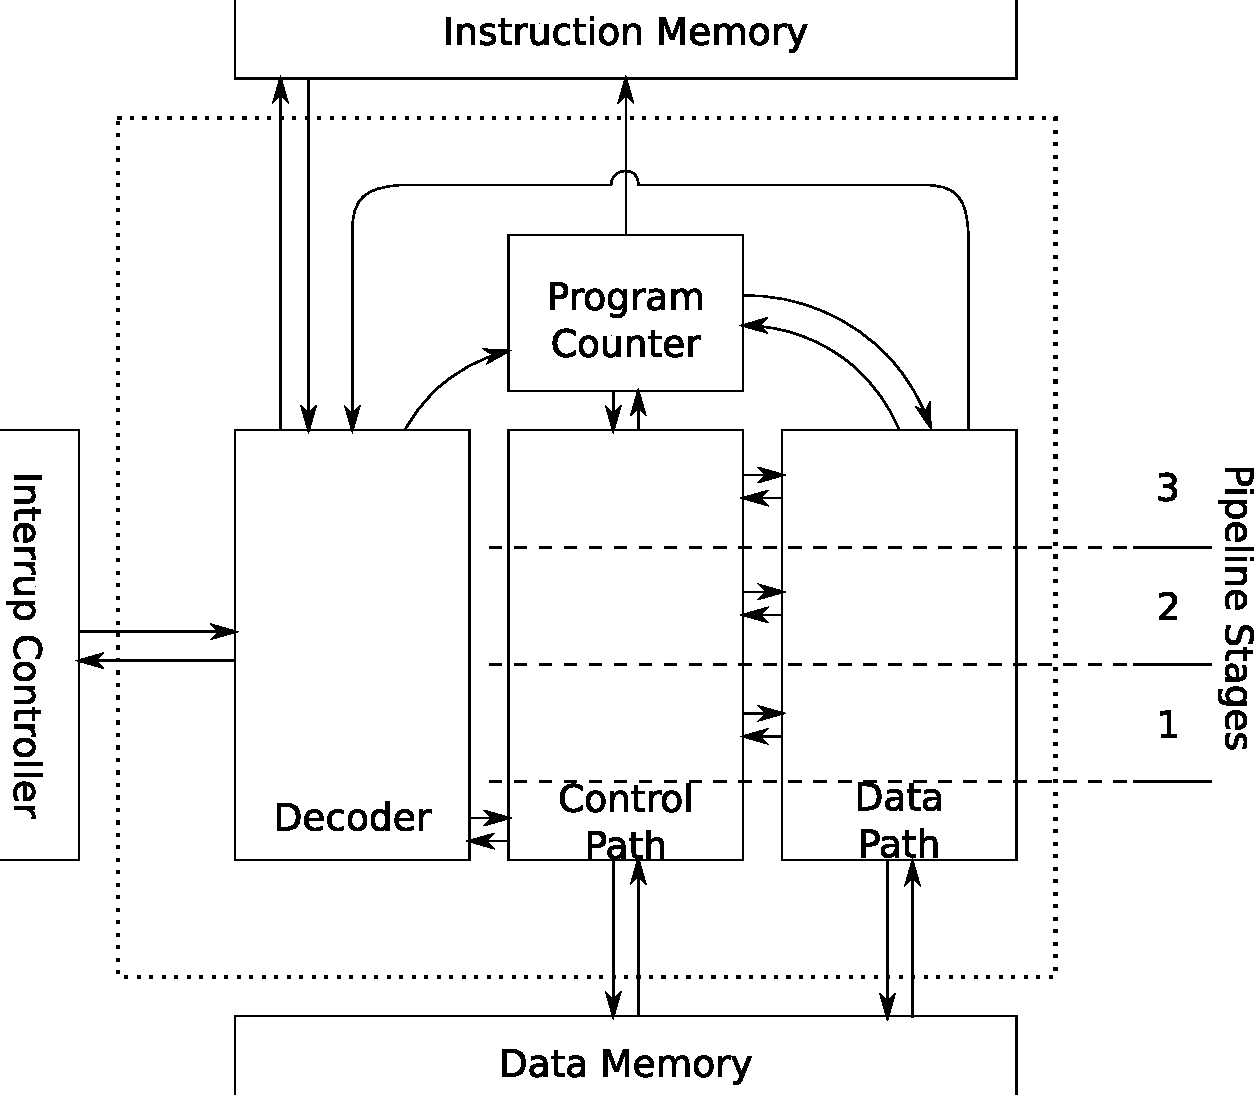
\includegraphics[scale=0.5]{./figures/block_core.pdf}
	\caption{Simplified Block diagram of core architecture with surrounding entities}
	\label{fig:blockdiagram_core}
\end{figure}
\begin{sidewaysfigure}[htb]
	\centering
	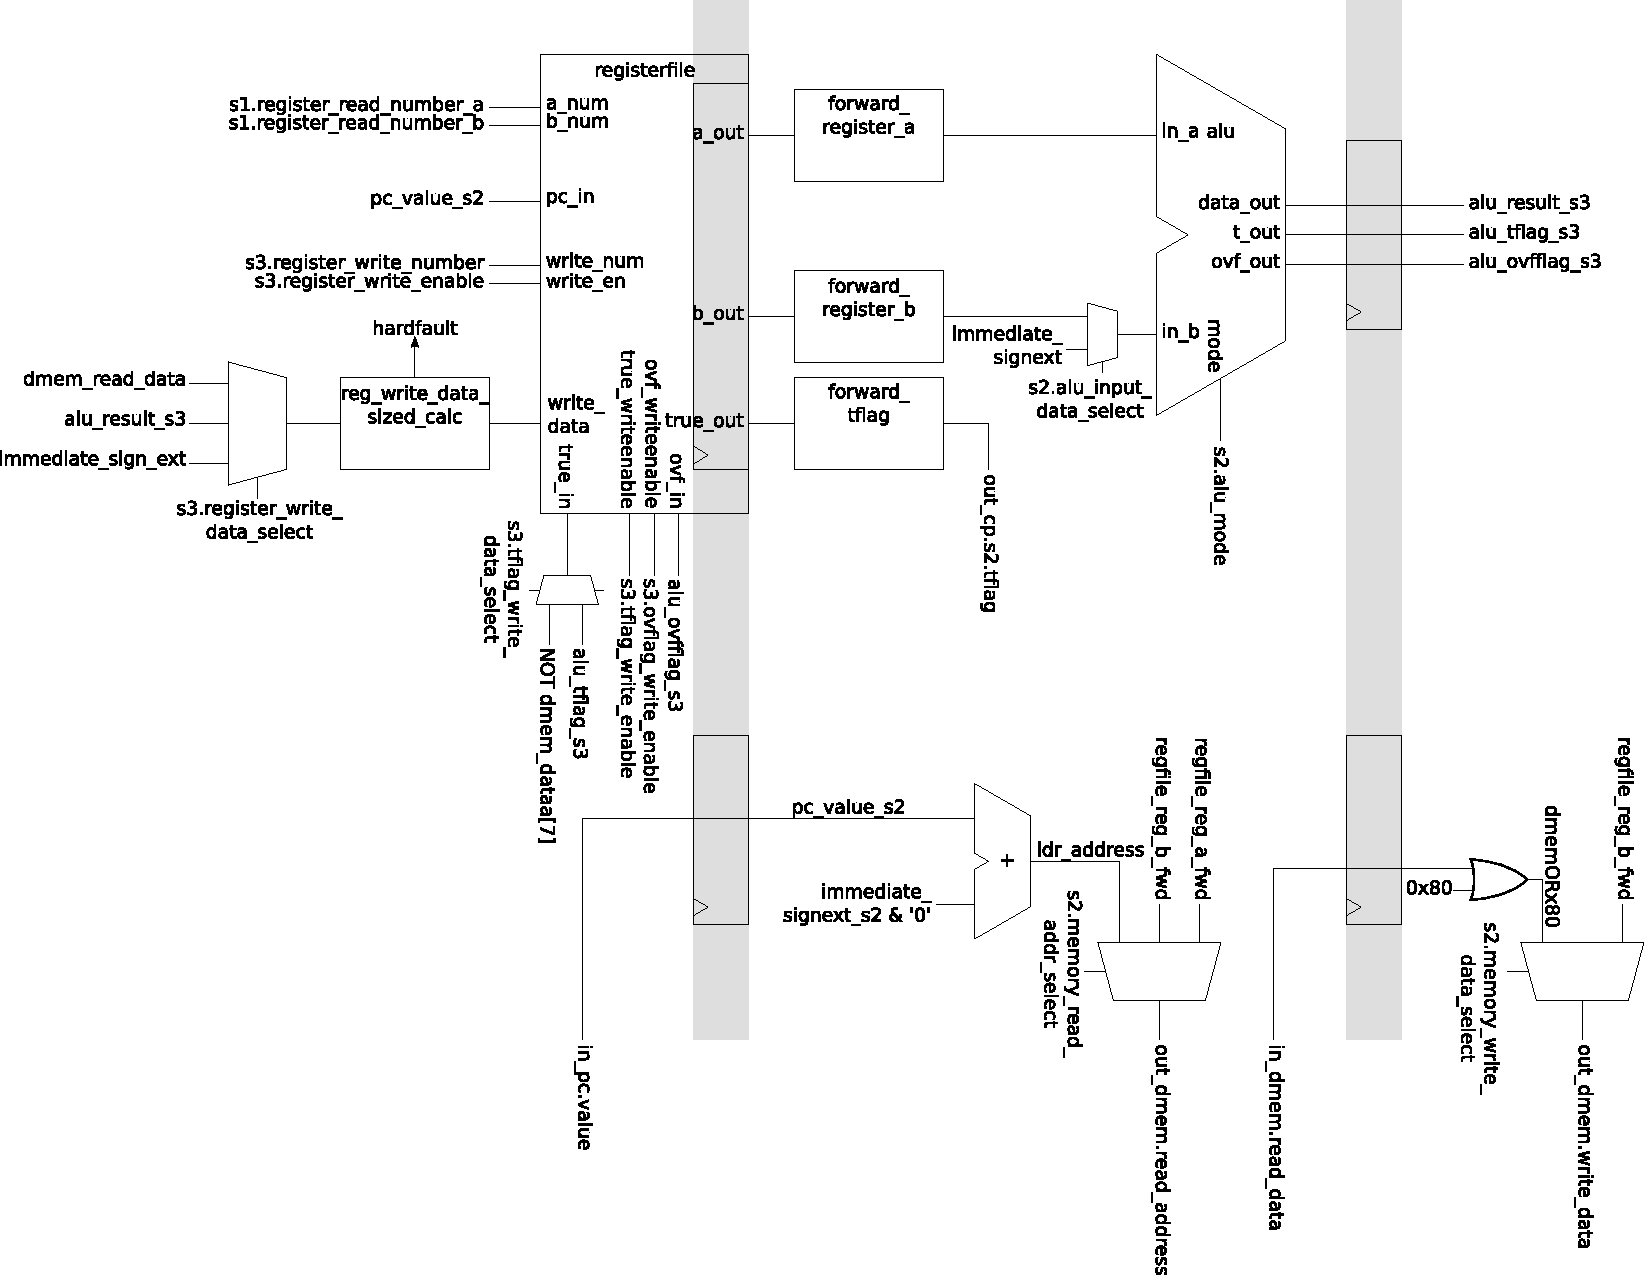
\includegraphics[scale=0.6]{./figures/block_dp.pdf}
	\caption{Block diagram of the datapath}
	\label{fig:blockdiagram_dp}
	Pipeline registers in gray, for reasons of clarity, not all signals are included.
\end{sidewaysfigure}

\section{Configuration}
\label{sec:config}
Easy ways to configure the \procname can be found in package \inlinevhdl{lt16x32\_internal} (see Listing \ref{lst:configcode_internal}) and in package \inlinevhdl{lt16x32$\_$global} (see Listing \ref{lst:configcode_global}).

\begin{vhdl}[Possible Configurations in internal package]{lst:configcode_internal}
-- execute branch delay slot. if set to true,
-- the first operation behind any type of branch
-- is executed. if set to false, stalls are inserted
constant execute_branch_delay_slot : boolean := TRUE;
-- register width
constant reg_width                 : integer := 32;
-- pc width (should be smaller or equal to register width)
constant pc_width                  : integer := 32;
\end{vhdl}

\begin{vhdl}[Possible Configurations in global package]{lst:configcode_global}
-- width of the vector holding the interrupt
-- number, maximum 7 due to processor architecture
constant irq_num_width             : integer := 4;
-- width of the vector holding the interrupt
-- priority, maximum 6 due to processor architecture
constant irq_prio_width            : integer := 4;
\end{vhdl}

Currently, three values can be configured:
\paragraph{Branch delay slot}
\label{sec:branchdelayslot}
If the constant \inlinevhdl{execute$\_$branch$\_$delay$\_$slot} is set to \inlinevhdl{true}, the instruction behind a branch instruction is always executed.
If the constant is set to \inlinevhdl{false}, a \inlineasm{nop} is inserted if a branch is performed.
By default, the branch delay slot is always executed.

Pay attention that even if the branch is not yet taken in the branch delay slot, the program counter may contain the new address.
Hence, instructions using the program counter should not be placed in the branch delay slot.
This also means, that storing the current address for function returns can not be done in the branch delay slot.
Instead, use the \inlinevhdl{call} instruction for this purpose.
\paragraph{Register width}
With the constant \inlinevhdl{reg$\_$width} the width of the internal registers can be set. Valid values are 8, 16 and 32, by default 32bits are used.
\paragraph{PC width}
With the constant \inlinevhdl{pc$\_$width} the width of the program counter can be set.
Valid values are 8, 16 and 32, it must be smaller or equal to the register width.
By default, 32bits are used.
\paragraph{Interrupt Number Width}
This constant holds the width of the interrupt number, values between 1 and 7 are valid.
This determines the number of possible interrupts.
By default, 4bits are used, allowing $2^4 = 16$ interrupts. 
\begin{equation*}
\text{Possible Interrupts} = 2^{(\text{Width})}
\end{equation*}
\paragraph{Interrupt Priority Width}
\label{sec:config_priowidth}
This constant determines the width of the runtime/interrupt priority, values between 1 and 6 are valid.
By default, 16 levels of priority are allowed.
One additional bit is supported by the use of non-maskable interrupts (NMI, see Section \ref{sec:nmi}).

\section{Pipeline Stages}
As shown in Figure \ref{fig:blockdiagram_dp}, the processor has three pipeline stages.
Due to this scheme, there is a delay between reading the instruction and changing data in the (register) memory of three clock cycles.

\paragraph{Stage 1: Decode/Setup}
In the first stage, the instruction is fetched from the instruction memory and decoded. Also, the needed register contents are loaded from the register file.
\paragraph{Stage 2: Load and Execute}
In this stage, the ALU is performing the operation and data is read from the data memory.
\paragraph{Stage 3: Writeback}
Data is written back to the register file and written to the data memory.
Possible sources for this data are the data read from the memory in the last clock cycle or the contents of register b.

\section{Registers}
The \procname has 16 registers, 14 of which can be used as general purpose registers.
The other four have special functions, VHDL defines are given in Listing \ref{lst:vhdl_regnumbers} and can be found in the \inlinevhdl{lt16x32\_internal} package.

\begin{vhdl}[Constant Defines for the Special Purpose Registers]{lst:vhdl_regnumbers}
-- register number for stack pointer
constant sp_num : reg_number := to_reg_number(12);
-- register number for link register
constant lr_num : reg_number := to_reg_number(13);
-- register number for status register
constant sr_num : reg_number := to_reg_number(14);
-- register number for pc register
constant pc_num : reg_number := to_reg_number(15);
\end{vhdl}

\subsection{General Purpose Registers}
Registers \inlineasm{r0} to \inlineasm{r11} can be used without special consideration as general purpose registers.
Registers \inlineasm{r12} (stack pointer) and \inlineasm{r13} (link register) can also be used as general purpose register but are additionally altered with special instructions.
\subsection{Stack Pointer}
The stack pointer (\inlineasm{r12}) is used when jumping into or out of interrupt handlers (i.e. external interrupts or \inlineasm{trap} instructions and \inlineasm{reti}).
It must be set to the correct address of the stack, before any interrupt is allowed to occur.
In the default configuration, stack grows downwards.
The stack pointer should be word-aligned at all times.

The interpretation of the stack pointer is always 'The current stack pointer points to the topmost element on the stack'.
When interfacing the stack pointer manually, always adhere to the following rules:
\begin{itemize}
\nolistskip
\item When writing to the stack (push), always decrement the stack before writing your element.
\item When reading from the stack (pop), read your element, then increment the stack pointer.
\end{itemize}
Only when adhering to these rules the integrity of the stack can be ensured.

The initial stack pointer position does not need to be a memory address,
but the word address below it needs to be valid.

\subsection{Link Register}
The link register (\inlineasm{r13}) is set by the \inlineasm{call} instruction.
This allows for flexible function returns using the pseudo instruction \inlineasm{ret} (a branch to the link register).
\subsection{Status Register r14}
The status register is a special 32bit register.
The register contents are displayed in table \ref{tbl:SR}, reserved bits always read zero and should be written to as zeroes for future compatibility.
\begin{table}
\center
\begin{tabular}{|c|c|c|c|c|c|c|c|c|c|c|c|c|c|c|c|}
\hline 
31 & 30 & 29 & 28 & 27 & 26 & 25 & 24 & 23 & 22 & 21 & 20 & 19 & 18 & 17 & 16\\ 
\hline 
\multicolumn{16}{|c|}{reserved}\\
\hline
\multicolumn{16}{c}{}\\
\hline 
15 & 14 & 13 & 12 & 11 & 10 & 9 & 8 & 7 & 6 & 5 & 4 & 3 & 2 & 1 & 0 \\
\hline 
\multicolumn{8}{|c|}{reserved} & \multicolumn{6}{|c|}{priority} & T & O \\
\hline
\end{tabular}
\caption{Status Register Contents}
\label{tbl:SR}
\end{table}

\subsubsection{Runtime Priority - SR[7-2]}
Bits seven to two define the current runtime priority, larger numbers mean higher priority. The priority is left aligned.
With a runtime priority width configured to four bits, the priority is stored in bits seven to four and the other bits read zero.
Writes to not used priority bits are discarded.

\subsubsection{Truthflag - SR[1]}
Bit one is the truth flag, which can be set/reset by compare instructions and are used for conditional branches and calls.
Also, the truth flag can be set manually by writing to the status register.

\subsubsection{Overflowflag - SR[0]}
Bit zero is the overflow flag, which is set by arithmetic instructions, such as addition and subtraction.

In additions an overflow has occured, if both operands are the same sign and the result's sign is different (i.e. $5 + 6 < 0$ or $(-5) + (-7) > 0$, listing \ref{lst:ovf_add}).
In subtractions an overflow occured, if both operands are from opposing sign and the minuend's sign differ from the result's (i.e. $(-8) - 5 > 0$ or $5 - (-4) < 0$, listing \ref{lst:ovf_sub}).
This follows normal rules for signed calculations, which are as well used in other processor designs. 

\begin{vhdl}[Overflow Generation for Addition]{lst:ovf_add}
c_out <= (in_a(reg_width-1)     AND in_b(reg_width-1)
                                AND not result(reg_width-1))

      OR (not in_a(reg_width-1) AND not in_b(reg_width-1)
                                AND result(reg_width-1));	
\end{vhdl}
\begin{vhdl}[Overflow Generation for Subtraction]{lst:ovf_sub}
c_out <= (in_a(reg_width-1)     AND not in_b(reg_width-1)
                                AND not result(reg_width-1))

      OR (not in_a(reg_width-1) AND in_b(reg_width-1)
                                AND result(reg_width-1));
\end{vhdl}

\subsection{Program Counter}
Register \inlineasm{r15} is reserved for the program counter and is read only from the user interface. Write accesses are ignored. It may be altered with special instructions such as branch and call and in interrupt request situations by the processor itself.

\chapter{Assembler and Instructions}

\section{Processor Instructions}
The \procname features a RISC instruction set with 16bit instructions and is prepared to be extended with 32bit and allows multicycle instructions.
In 16bit instructions, the first nibble (4bits) of the instruction code is the opcode determining the operation.
The opcode \bits{1111} is reserved for 32bit instructions which are always are word aligned.

\subsection{Instruction Format}
Several different instruction formats are used in the \procname.
As at the moment, no 32bit instruction is implemented, this section describes instruction formats for 16bit instructions only.
Each halfword is split up into four nibbles (each of a size of 4bits), whose meaning can be seen in Table \ref{tbl:instr_formatnibbles}.

\begin{table}
\caption{16bit Instruction Formats}
\label{tbl:instr_formatnibbles}
\begin{center}
\begin{tabular}{|l||c|c|c|c||p{0.2\textwidth}|}
\hline
Format				& 15-12		& 11-8		& 7-4		& 3-0		& Example Uses\\
\hline\hline
Three Registers		& opcode		& Rd			& Ra			& Rb			& Calculations\\
\hline
4bit Immediate		& opcode		& Rd			& Ra			& Imm(3-0)	& Shift\\
\hline
8bit Immediate		& opcode		& Rd			& Imm(7-4)	& Imm(3-0)	& Add Immediate, Load PC-Relative\\
\hline
Mode	 with Register	& opcode		& Mode		& Ra			& Rb			& Compare, Load/Store\\
\hline
Mode	 with Immediate	& opcode		& Mode		& Imm(7-4)	& Imm(3-0)	& Branch/Call to Immediate\\
\hline
\end{tabular}
\end{center}
\end{table}

\subsection{List of available Instructions}
\label{sec:instructionlist}
The following instructions are supported:
\paragraph{Arithmetic Operations}
\begin{itemize}
\nolistskip
\item \hyperref[instr_add]{Signed Addition}
\item \hyperref[instr_sub]{Signed Subtraction}
\item \hyperref[instr_addi]{Signed Addition with Immediate}
\end{itemize}
\paragraph{Bitwise/Logic Operations}
\begin{itemize}
\nolistskip
\item \hyperref[instr_and]{Bitwise AND}
\item \hyperref[instr_or]{Bitwise OR}
\item \hyperref[instr_xor]{Bitwise XOR}
\item \hyperref[instr_lsh]{Logic Shift Left}
\item \hyperref[instr_rsh]{Logic Shift Right}
\item \hyperref[instr_cmp]{Compare}
\end{itemize}
\paragraph{Memory Operations}
\begin{itemize}
\nolistskip
\item \hyperref[instr_ldr]{Load PC Relative}
\item \hyperref[instr_ld]{Load Data from Pointer}
\item \hyperref[instr_st]{Store Data to Pointer}
\end{itemize}
\paragraph{Branch/Call/Trap Operations}
\begin{itemize}
\nolistskip
\item \hyperref[instr_bri]{Branch to Offset}
\item \hyperref[instr_brr]{Branch to Register}
\item \hyperref[instr_calli]{Call to Offset}
\item \hyperref[instr_callr]{Call to Register}
\item \hyperref[instr_trap]{Trap}
\item \hyperref[instr_reti]{Return from Interrupt}
\item \hyperref[instr_brt]{Branch to Table}
\end{itemize}
\paragraph{Miscellaneous Operations}
\begin{itemize}
\nolistskip
\item \hyperref[instr_tst]{Test and Set}
\end{itemize}

\instruction{Signed Addition}{add}
	{0011 dddd aaaa bbbb}
	{add rd, ra, rb}
	{Registers ra and rb are treated as two signed numbers and are added. The result is stored in rd.}
	{rd = ra + rb;}
	{The overflow flag is updated.}

\instruction{Signed Subtraction}{sub}
	{0001 dddd aaaa bbbb}
	{add rd, ra, rb}
	{Registers ra and rb are treated as two signed numbers and are subtracted. The result is stored in rd.}
	{rd = ra - rb;}
	{The overflow flag is updated.}
	
\instruction{Bitwise AND}{and}
	{0010 dddd aaaa bbbb}
	{and rd, ra, rb}
	{Registers ra and rb are treated as bit masks and are anded with each other. The result is stored in rd.}
	{rd = ra \& rb;}
	{No flag is updated.}

\instruction{Bitwise OR}{or}
	{0000 dddd aaaa bbbb}
	{or rd, ra, rb}
	{Registers ra and rb are treated as bit masks and are ored with each other. The result is stored in rd.}
	{rd = ra | rb;}
	{No flag is updated.}

\instruction{Bitwise XOR}{xor}
	{0100 dddd aaaa bbbb}
	{xor rd, ra, rb}
	{Registers ra and rb are treated as bit masks and are xored with each other. The result is stored in rd.}
	{rd = ra $\hat\ $ rb;}
	{No flag is updated.}
	
\instruction{Logic Shift Left}{lsh}
	{0101 dddd aaaa bbbb}
	{lsh rd, ra, imm}
	{Register ra is treated as bit masks and shifted to the left by imm bits, ra is filled with zeroes. imm is treated as unsigned number. The result is stored in rd. Internally, imm is incremented by one, which is compensated for in the assembler.}
	{rd = ra $<<$ imm;}
	{No flag is updated.}
	
\instruction{Logic Shift Right}{rsh}
	{0110 dddd aaaa bbbb}
	{rsh rd, ra, imm}
	{Register ra is treated as bit masks and shifted to the right by imm bits, ra is filled with zeroes. imm is treated as unsigned number. The result is stored in rd. Internally, imm is incremented by one, which is compensated for in the assembler.}
	{rd = ra $>>$ imm;}
	{No flag is updated.}

\instruction{Signed Addition with Immediate}{addi}
	{0111 dddd iiii iiii}
	{addi rd, imm}
	{Register rd and imm are treated as signed numbers and are added. The result is stored in rd.}
	{rd = rd + imm;}
	{The overflow flag is updated.}

\instruction{Compare}{cmp}
	{1000 mmmm aaaa bbbb}
	{cmp mode ra, rb}
	{Registers ra and rb are treated as signed numbers and are compared. If the condition, given by mode is true, the truth-flag is set, otherwise reset. Allowed modes are\begin{description}\nolistskip
	\item[0000, eq]equal
	\item[1000, neq]not equal
	\item[0010, gg]greater
	\item[0001, ge]greater or equal
	\item[1001, ll]less
	\item[1010, le]less or equal
	\end{description}}
	{(ra == rb) ? (T=1) : (T=0);\\// where == is interchangable by mode}
	{The truth flag is updated.}

\instruction{Load PC Relative}{ldr}
	{1010 dddd iiii iiii}
	{ldr rd, imm}
	{Register rd is loaded with memory data from address (PC+(imm$<<$1)), where imm is treated as signed number and is left shifted by one bit.}
	{rd = *(PC + (imm$<<$1)}
	{No flag is updated.}

\instruction{Load Data from Pointer}{ld}
	{1011 0mmm aaaa bbbb}
	{ld08 ra, rb\\ld16 ra, rb\\ld32 ra, rb}
	{Loads data from pointer. Register rb's content is used as absolute address, the loaded data is written to register ra. Following modes are supported:
	\begin{description}
	\nolistskip
	\item[000] Load byte
	\item[001] Load halfword
	\item[010] Load word
\end{description}		
	}
	{ra = *rb}
	{No flag is updated}
	
\instruction{Store Data to Pointer}{st}
	{1011 1mmm aaaa bbbb}
	{st08 ra, rb\\st16 ra, rb\\st32 ra, rb}
	{Stores data to pointer. Register ra's content is used as absolute address to store the content of register rb. Following modes are supported:
	\begin{description}
	\nolistskip
	\item[000] Store byte
	\item[001] Store halfword
	\item[010] Store word
\end{description}
	As the data is valid only after two clock cycles, the user must ensure that the same address is not used in read transactions in the following instruction (such as ld, ldr, tst). 
	}
	{*ra = rb}
	{No flag is updated}

\instruction{Branch to Offset}{bri}
	{1100 010c iiii iiii}
	{br imm\\br always/true imm}
	{Sets the program counter to PC+imm, where imm is treated as signed number. For details about the branch delay slot see section \ref{sec:branchdelayslot}. If c==1, the branch is conditional and performed only, if the truth flag is set.}
	{if ((c==0) \logicor (T==1)) goto (PC+imm$<<$1);}
	{No flag is updated}

\instruction{Branch to Register}{brr}
	{1100 011c aaaa xxxx}
	{br ra\\br always/true ra}
	{Sets the program counter to register a. For details about the branch delay slot see section \ref{sec:branchdelayslot}. If c==1, the branch is conditional and performed only, if the truth flag is set.}
	{if ((c==0) \logicor (T==1)) goto (ra$<<$1);}
	{No flag is updated}
	
\instruction{Call to Offset}{calli}
	{1100 100c iiii iiii}
	{call imm\\call always/true imm}
	{Sets the program counter to PC+imm, where imm is treated as signed number, and stores the current program counter in the link register. If c==1, the call is conditional and performed only, if the truth flag is set. This is a multicycle operation which consumes two clock cycles.}
	{if ((c==0) \logicor (T==1)) \{LR=PC; goto (PC+imm);\}}
	{No flag is updated}
	
\instruction{Call to Register}{callr}
	{1100 101c aaaa xxxx}
	{call ra\\call always/true ra}
	{Sets the program counter to register a and stores the current program counter in the link register. If c==1, the call is conditional and performed only, if the truth flag is set. This is a multicycle operation which consumes two clock cycles.}
	{if ((c==0) \logicor (T==1)) \{LR=PC; goto (ra$<<$1);\}}
	{No flag is updated}

\instruction{Trap}{trap}
	{1100 11xx iiii iiii}
	{trap imm}
	{Request an interrupt of number imm. Number of bits for imm can be set in processor configuration, the number must be right aligned.}
	{no equivalent}
	{No flag is updated}

\instruction{Return from Interrupt}{reti}
	{1100 000x xxxx xxxx}
	{reti}
	{Returns from Interrupt, by popping the link and status register from the stack and branching to the current link register contents. This is a multicycle operation which consumes five clock cycles.}
	{no equivalent}
	{No flag is updated.}

\instruction{Branch to Table}{brt}
	{1100 001c aaaa xxxx}
	{brt ra}
	{Increments the program counter by register a. This allows for easy creation of branch tables. For details about the branch delay slot see section \ref{sec:branchdelayslot}. If c==1, the branch is conditional and only performed if the truth flag is set.}
	{PC = PC + (ra$<<$1)}
	{No flag is updated.}

\instruction{Test and Set}{tst}
	{1001 dddd aaaa xxxx}
	{tst rd, ra}
	{Test and set can be used to implement mutexes. The lower seven bits of the byte can be used to implement semaphores.}
	{temp=$_\text{byte}$*ra; rd = temp;\\T = (temp \& 0x80==0); temp=temp $|$ 0x80; *ra=$_\text{byte}$temp;}
	{The T-flag is set if the mutex is free and reset if the mutex is already reserved.}

\section{Assembler}

The supplied assembler is a two-pass assembler (see thesis, Section 2.6) based on \filename{flex} and \filename{bison} which are used to parse the input file.

\subsection{HowTo: Assemble Input Files}
A prepared assembler file \filename{input.prog} (see examples in \filename{/source/programs/}) can easily assembled into a formatted file \filename{output.ram} supported by the \procname by calling the assembler \filename{asm}:
\begin{verbatim}
asm input.prog -o output.ram
\end{verbatim}

\subsection{Allowed Input}
The input to the assembler is case sensitive and all mnemonics have to be lower case. A typical line follows Listing \ref{lst:asm_general}, where all parts are optional (a mnemonic is needed if parameters are supplied though).

\begin{asm}[General Inputline]{lst:asm_general}
label: mnemonic mode par1, par2, par3 // comment
\end{asm}

Parameters can either be registers names r0 to r15, SP, LR, SR or PC,
or can be immediate values in various number formats (decimal, binary or hexadecimal numbers),
for prefixes see Table \ref{tbl:asm_numberformats}.
Binary and hexadecimal numbers are not sign extended and always treated as unsigned values.
Also, absolute or relative references to labels are allowed as parameters, see Section \ref{sec:labels} for details.

Number and type of parameters vary for each instruction, allowed combinations are listed in Section \ref{sec:instructionlist}.

\begin{table}
	\begin{center}
	\begin{tabular}{|c|c|c|}
	\hline 
	Numberformat & Prefix & Example\\
	\hline\hline
	Decimal      & None   & -45 \\ 
	Binary       & 0b     & 0b11011 \\ 
	Hexadecimal  & 0x     & 0xFE \\ 
	\hline 
	\end{tabular} 
	\end{center}
	\caption{Number Format Prefixes}
	\label{tbl:asm_numberformats}
\end{table}

\subsection{Pseudo Instructions}
Several instructions are supported which are not directly processed by the \procname but which are mapped to other instructions.
For details on the instructions used, see Section \ref{sec:instructionlist}.
\begin{description}
\item[No Operation (nop)] No operation is performed, wait one clock cycle. Mapped to \inlineasm{or r0, r0, r0}.
\item[Move Register (mov rd, ra)] The content of \inlineasm{ra} is copied to \inlineasm{rd}. Mapped to \inlineasm{or rd, ra, ra}.
\item[Return (ret)] Returns to callee after a call instruction. Mapped to \inlineasm{br always lr}.
\item[Clear Register (clr rd)] Resets \inlineasm{rd} to zero. Mapped to \inlineasm{xor rd, rd, rd}.
\end{description}

\subsection{Directives}%
\label{sec:AssemblerDirectives}%
The assembler supports several directives which can be included in the input code, see Listing \ref{lst:asm_directives}.
\begin{description}
\item[.word]stores the following parameter directly into the memory.
\item[.address]inserts nops until the address given as parameter is reached.
\item[.align]if needed, a 16bit nop is inserted to align the following instruction
\end{description}

\begin{asm}[Example for the use of directives]{lst:asm_directives}
// load variables from constant pointer
           ldr     r0,    >variableA
           ldr     r1,    >variableB

// store variableA           
           .align       // fix eventual non-word-alignment
variableA: .word 0x1234

// store variableB
           .address 0x100 // store variableB at address 0x100
variableB: .word    0xABCD
\end{asm}

\subsection{Labels}
\label{sec:labels}
Labels can be set in the code directly, as seen in Listing \ref{lst:asm_general}.
They can be reffered to in absolute or relative manner (see Listing \ref{lst:asm_labels}).
Label names can include upper and lower case letters, numbers and underscores.
While absolute referencing puts the whole address into the output, relative referencing adds only the difference to the address of instruction which is referencing to the label.
\begin{asm}[Label References]{lst:asm_labels}
label:  br   >label // relative reference
       .word =label // absolute reference
\end{asm}

\subsection{Assembler Options}
Several command line options are available:
\begin{description}
\item[-o filename]Determines the output file.
\item[-m filename]The assembler outputs a map file, containing all labels and their addresses.
\item[-v or -\xspace -verbose]Outputs all intermediate information.
\item[-\xspace -autoalign]Automatically aligns 32bit instruction and immediate values
\item[-\xspace -fillbds]Fills branch delay slots with nop instruction (i.e. inserts nop after all branches)
\item[-\xspace -continue-on-error]Continues parsing even with errors.
\end{description}

\subsection{Output}
The standard output format is a one-word-per-line bitstring representation of the instruction memory, which can directly be read by the testbench provided and used as input for memory synthesis.

\section{HowTo: Add more instructions}
\subsection{Processor Side}
\begin{enumerate}
\item Add opcode constant define to \verb=lt16x32_internal= package.
\item Add case to 16bit decoder and set control signals that differ from default settings.
\end{enumerate}
\subsection{Assembler Side}
\begin{enumerate}
\item Add enumerate item to op$\_$t in global.h
\item Add pattern to flex code in asm.l
\item Add handling to handle$\_$xy.c according to wished syntax style.
\item Recompile assembler by running the make script.
\end{enumerate}
\subsection{32bit Extension}
If 32bit instruction should be implemented, follow the structure of the 16bit decoder to implement the 32bit decoder in \filename{decoder\_32bit.vhd}.

\subsection{Multicycle Instructions}
To implement multicycle operations, changes need to be implemented in \filename{decoder$\_$fsm.vhd}.
Use the implementation of \textit{reti} as an example.


\chapter{Interrupts}
\section{Interrupt Controller}
\label{sec:irq_ctrl}
The interrupt controller features a configurable number of interrupt lines with a configurable amount of priorities.
The configuration follows that of the \procname (see Section \ref{sec:config}).
These intterupts lines need to be asserted for one clock cycle to trigger an interrupt request to the processor core.
Additionally, trap requests from the core are handled (as described in \ref{sec:trap}).

\section{Priority, NMI}
\label{sec:nmi}
The processor features multiple levels of runtime priority (configurable, see Section \ref{sec:config_priowidth}) where a greater number means higher priority.
Additionally, non maskable interrupts (NMI) are supported which are always executed regardless the current processor runtime priority.

The processor starts with the highest possible runtime priority by default to disable interrupts at startup (with the exception of NMI).

This is needed as the stack pointer needs to be set to a valid address before any interrupt (including NMI) can be executed.

\section{Interface and Timing Diagram}
Both ports \inlinevhdl{in\_irq} and \inlinevhdl{out\_irq} (for type definitions see Listing \ref{lst:typedef_irq}) should be connected to a fitting interrupt controller (for example the implementation described in Section \ref{sec:irq_ctrl}).

\begin{vhdl}[Type definitions for Interrupt Controller Ports]{lst:typedef_irq}
-- collection of all signals from the
-- interrupt controller to the core
type irq_core is record
	-- interrupt number of requested interrupt
	num      : unsigned(irq_num_width - 1 downto 0);
	-- priority of requested interrupt
	-- (higher number means higher priority)
	priority : unsigned(irq_prio_width - 1 downto 0);
	-- request signal, active high
	req      : std_logic;
	-- non maskable interrupt flag, active high
	nmi      : std_logic;
end record;

-- collection of all signals from the core
-- to the interrupt controller
type core_irq is record
	-- interrupt acknowledge
	-- high if requested interrupt is processed
	ack      : std_logic;
	-- number of interrupt requested by
	-- internal trap instruction
	trap_num : unsigned(irq_num_width - 1 downto 0);
	-- request signal for internal trap, active high
	trap_req : std_logic;
end record;
\end{vhdl}

\subsection{Interrupt Request}
The external world (i.e. the interrupt controller) can request an interrupt by writing the interrupt number, its priority to \inlinevhdl{in\_irq} and setting the \inlinevhdl{nmi} bit accordingly.
After these are set, \inlinevhdl{req} can be asserted and must be held high until the core acknowledges the interrupt request by asserting \inlinevhdl{ack} for one clock cycle (see Figure \ref{fig:signal_irq_req}).

\begin{figure}[htb]
	\center
	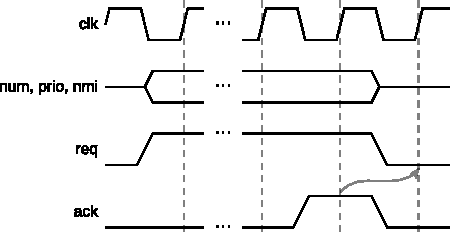
\includegraphics[scale=1]{./figures/signal_irq_req.pdf}
	\caption{Signal Pattern for Interrupt Requests}
	\label{fig:signal_irq_req}
\end{figure}

\subsection{Trap Implementation}
\label{sec:trap}
When executing a trap instruction, an interrupt line to the interrupt controller is asserted for one clock cycle with the interrupt number asserted as well, see Figure \ref{fig:signal_irq_trap}.
Note, that an arbitrary time (and number of instructions) may take place between a trap and the interrupt handler execution.
\begin{figure}[htb]
	\centering
	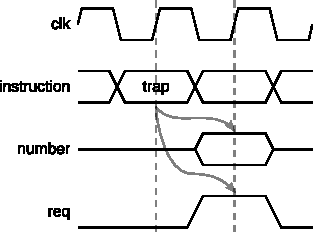
\includegraphics[scale=1]{./figures/signal_irq_trap.pdf}
	\caption{Signal Pattern for Trap Instruction}
	\label{fig:signal_irq_trap}
\end{figure}

\subsection{Processor Interrupt Behavior}
\label{sec:InterruptEntryCPU}
When an interrupt is accepted by the processor, it saves the current PC and status register on the stack.
Then it replaces the runtime priority in the status register with interrupt's priority and replaces the PC with the interupt vector number.

The \textit{reti} instruction reverses this and resturn to the previous executed program.
Note that the processor by itself does not save any registers apart from status register and program counter.
Any other register that needs to be preserved needs to be saved manually.

\chapter{Memory}

The \procname is connected to the memory through a harvard architecture style interface.
While the interface to the instruction memory is read only, the data memory interface must handle read and write transactions simultaneously.
Externally, both instruction and data memory can be mapped to a Von-Neumann architecture.
The implemented Harvard architecture is more general and allows for two caches to be implemented.

\section{Endianess and Memory Width}
The memory width is defined in the \inlinevhdl{lt16x32\_internal} package.
Currently, memory widths of 32bits are supported only.
Of course, this memory width can be mapped to any other memory width by a memory controller.
The memory organizes data in big endian format.
This can be seen (and changed) in the memory controller, Listing \ref{lst:endianess}.
The same is valid for halfword-accesses.

\begin{vhdl}[Byte-Order in Memory]{lst:endianess}
case byteaddress is
when "00" =>
	dmem_data(7 downto 0) <= word(7 downto 0);
when "01" =>
	dmem_data(7 downto 0) <= word(15 downto 8);
when "10" =>
	dmem_data(7 downto 0) <= word(23 downto 16);
when "11" =>
	dmem_data(7 downto 0) <= word(31 downto 24);
\end{vhdl}

\section{Interface and Timing Description}
\subsection{Instruction Memory Interface}
The \procname is connected to the instruction memory through two ports, as seen in Listing \ref{lst:imem_interface}.
Their datatype definitions can be found in the \inlinevhdl{lt16x32\_global} package.
\begin{vhdl}[Instruction Memory Interface]{lst:imem_interface}
entity core is
port(
	[...]
	-- signals from instruction memory
	in_imem   : in  imem_core;
	-- signals to instruction memory
	out_imem  : out core_imem;
	[...]
);
end entity core;
\end{vhdl}

\subsubsection{Read Access}
As all clocked signals in this design, the address and data signals to the instruction memory must be read on each rising clock edge.
Data must be provided if enable (\inlinevhdl{en}) is asserted and the memory content is read on the next rising clock edge.
This single data rate scheme allows for double data rate memory access to allow for pseudo-simultaneous data and instruction memory access.
A standard signal pattern can found in Figure \ref{fig:signal_imem}.

\begin{figure}[htb]
\centering
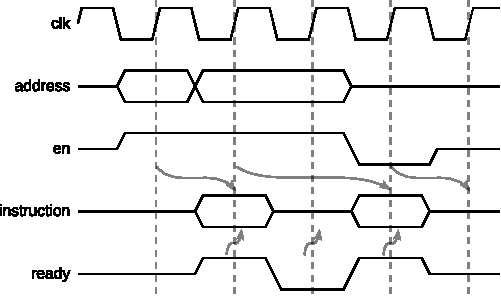
\includegraphics[scale=1]{./figures/signal_imem.pdf}
\caption{Signal Pattern for the Instruction Memory Interface}
\label{fig:signal_imem}
\end{figure}

\subsection{Data Memory Interface}
The \procname is connected to the data memory through two ports, as seen in Listing \ref{lst:dmem_interface}, their datatype definitions can be found in the \inlinevhdl{lt16x32\_global} package.
The data memory interface must be able to handle simultaneous read and write accesses, as these are performed in different pipeline stages and can overlap.
This is good for memory transaction performance but introduces a high memory load.

\begin{vhdl}[Data Memory Interface]{lst:dmem_interface}
entity core is
port(
	[...]
	-- signals from data memory
	in_dmem   : in  dmem_core;
	-- signals to data memory
	out_dmem  : out core_dmem;
	[...]
);
end entity core;
\end{vhdl}

\subsubsection{Read Access}
The read access to the data memory is similar to the instruction memory interface and a standard signal pattern is shown in Figure \ref{fig:signal_imem}.

\subsubsection{Write Access}
In a write access, data and address are supplied at the same time and should be copied to the memory at the rising clock edge if enable is active, see Figure \ref{fig:signal_dmem_write}.
\begin{figure}[htb]
	\centering
	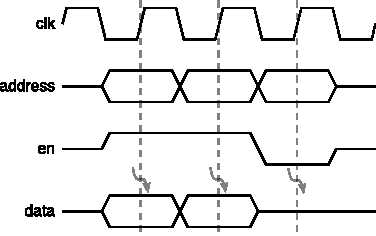
\includegraphics[scale=1]{./figures/signal_dmem_write.pdf}
	\caption{Signal Pattern for Data Memory Write}
	\label{fig:signal_dmem_write}
\end{figure}
\subsection{Memory Bandwidth Solutions}
As mentioned before, the very liberal memory interface demands high memory bandwidth.
In a worst-case scenario three memory accesses are needed per clockcycle (instruction read, data read and data write).

\subsubsection{Instruction Alignment}
Fortunately this worst-case scenario can be avoided by clever instruction alignment.
As standard instructions are 16bit wide and the instruction memory is organized
in 32bit words the instruction memory must be read only once every two clock cycles\footnote{Branching may introduce additional read operations.}.
If memory access instructions are now aligned in such a way, that read/write actions are performed when the instruction memory is idle, a simple single data rate memory is sufficient.
An exemplatory signal pattern is shown in Figure \ref{fig:signal_mem_interlacing}.
Note, that the instruction memory enable must be asserted the whole time,
but the memory controller does not need to read the actual memory,
as the address is changed only every second clock cycle.

\begin{figure}[htb]
	\centering
	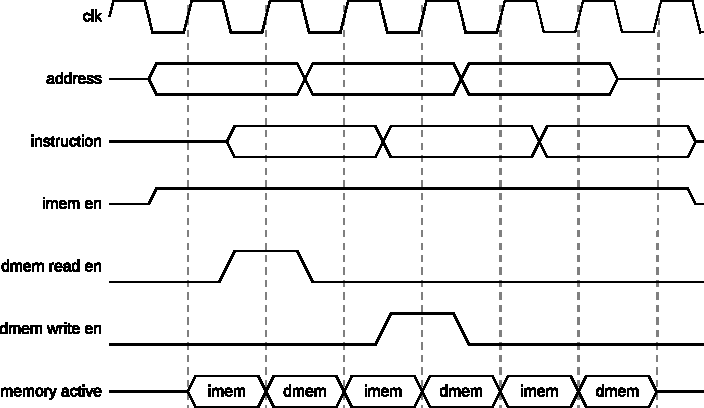
\includegraphics[scale=1]{./figures/signal_mem_interlacing.pdf}
	\caption{Signal Pattern for Memory Interlacing}
	\label{fig:signal_mem_interlacing}
\end{figure}

\subsubsection{Processor Stalling}
If instruction alignment is too cumbersome or the memory is too slow for any other reason, it can deassert the ready signal (\inlinevhdl{ready}) to the processor (per interface).
If \inlinevhdl{ready} is deasserted, the processor is stalled and waits for \inlinevhdl{ready} to become asserted again.

\section{Memory Mapped I/O}
\label{sec:memmappedio}
In the concept of memory mapped input/output (I/O), the processor core does not distinguish between data memory transactions and transactions with other kinds of devices.
Writing to special memory addresses (i.e. outside of the memory range) are forwarded to a device, reading from these addresses means accessing the device's registers.

The systems memory is defined as follows:
\begin{itemize}
\item The instruction memory starts at address zero, its length should be configured to a word boundary.\footnote{The default component uses is configured using a word count.}
\item The data memory starts after the instruction memory, its length is also configurable and should also end on a word boundary.
\item The address space of the peripheral components starts at address \verb=0x000F0000=
\end{itemize}

\section{Memory Controller}
\label{sec:memoryctrl}
A generic memory controller named \verb=dmem= is given.
It has a size of 256 bytes, sectioned in four 64 byte blocks with an access size of one byte.
The default configuration is that its base address is directly after the instruction memory.
It can and should be used to maintain the stack, as frequent accesses to the instruction memory can slow down the performance.
The content of the memory at startup is undefined, and should not be used without initialization.
\chapter{Guides}

\section{How to implement a lookup or branch table}
Due to the limitation of the \verb=ldr= instruction,
addressing large fields of constants with it is not feasible,
especially if those constants are refered to by more than one part of the program.

This can be circumvented by using the assemblers directive \verb|=labelname| to store a pointer to a labels location (See Section~\ref{sec:AssemblerDirectives}).
Pointers to data in memory can be stored conviently close to an \verb=ldr= instruction, 
making the access to the memory content via a pointer based load or store instruction possible.

The most common use of this mechanic is the lookup table.
An example is given in Listing~\ref{lst:ldr_useage}.

\begin{asm}[Example on indirect LDR use]{lst:ldr_useage}
.align
lookup_table:
    .word 0x0001
    .word 0x0010
//...
// large amounts of code and/or data
//...

.align
lookuptable_ptr: 
    .word =lookup_table
//...
    ldr rX , >lookuptable_ptr
//...
    ld32 rY,rX // load from pointer
    addi rX, 4
    ld32 rZ,rX // load from pointer with offset
//...
\end{asm}

\clearpage
\section{How to test a design using the CAN test package}
%Designs that use a CAN controller as a peripheral device, are often complex and therefor hard to debug. 
%This is especially true, if providing valid input data via the CAN bus is necessary in order to verify correct behavior.
The platform includes a foreign CAN controller IP component. 
To ease integration and testing, a test package is provided with the platform source code.
With its help, input data and behavior of a CAN network can be modeled more easily.

The test package is located in \verb=can_tp.vhd= and a application demonstration is given as a testbench in \verb=can_demo_tb.vhd= in the testbench directory.

In this guide, two approaches on verifying a design are presented.

%In those situations, the need for tools occurs, that reliably provide input data and model the behavior of a CAN network,
%connected to the designs CAN interface. 
%The CAN test package is a collection of VHDL functions and procedures that implement such tools. 
%And this guide will explain their proper use.

%There are two basic approaches, recommended by this guide, on how to do so. 
%They are described in the two following parts. 
%The third part gives some hints on how to use these methods in a test bench.



\subsection{Simulating a CAN transmission}
The first approach focuses on generating CAN transmissions, that can be used as input for the design under test. This is achieved by unsing the procedure \verb=simulate_can_transmission= (Listing ~\ref{lst:interface_01}), which is configurable to any data and timing, your CAN interface uses. The user has not to worry about bit stuffing, crc and error detection.

The \verb=id= and \verb=data= parameters are bit vectors (\verb=std_logic_vector=) that specify the CAN ID and DATA bits of the message.

The actual length of the data part is configurable by the \verb=datasize= parameter. It is an integer specifying the amount of Bytes of the \verb=data= parameter, that will be included in the CAN transmission. The rest of \verb=data= will simply be ignored.

The timing is controlled by the \verb=t_bit= parameter, which is of VDHL type time.
It stands for the correct overall length of one CAN symbol (this value has to be calculated from the timing configuration of the tested CAN controller).

The \verb=rx= and \verb=tx= signals have to be connected to a simulated CAN bus. See Section ~\ref{subsec:int_tb} for more information. The signal \verb=tx= is the actual output of the procedure.

The \verb=test_result= parameter is a diagnostic output of an enumeration type that shows whether the transmission was successful, a CAN error occurs, the arbitration is lost or whether the tested CAN controller is not acknowledging the transmission.

\begin{vhdl}[Interface]{lst:interface_01}
procedure simulate_can_transmission(
        constant id 		: in std_logic_vector(10 downto 0);
        constant data		: in std_logic_vector (0 to 63);
        constant datasize	: in integer;
        constant t_bit		: in time;
        signal rx			: in std_logic;
        signal tx			: inout std_logic;
        signal test_result	: out rx_check_result)
\end{vhdl}

\subsection{Creating a test network}
While the first approach is limited to transmitting can messages, this one aims at providing one or more fully functioning can nodes in a test network. Each node is implemented by an instantiation of \verb=can_vhdl_top=, but instead of steering them with a LT16soc design, functions of the can test package will do the job:

If a certain register in a CAN node should be written to, the procedure \verb=can_wb_write_reg= (Listing ~\ref{lst:interface_02}) comes in handy. Its parameter signals \verb=wbs_in= and \verb=wbs_out= must be connected to the CAN controller's Wishbone interface. The parameter \verb=addr= is an integer specifying the target register of the write and the parameter data is a bit vector containing the data. And finally a clock signal \verb=clk= is needed as input, in order to write to the CAN controller. (This must be the same clock used for operating the CAN node.)

\begin{vhdl}[Interface]{lst:interface_02}
procedure can_wb_write_reg(
        signal wbs_in 	: out wb_slv_in_type;
        signal wbs_out 	: in wb_slv_out_type;
        constant addr 	: integer;
        constant data	: in std_logic_vector(7 downto 0);
		signal clk 		: in std_logic)
\end{vhdl}

For extracting certain register contents, the procedure \verb=can_wb_read_reg= (Listing ~\ref{lst:interface_03}) is provided. It is used with the same parameters like \verb=can_wb_write_reg=, except a data input bit vector. Instead, a data output signal is provided, to access the read register contents.

\begin{vhdl}[Interface]{lst:interface_03}
procedure can_wb_read_reg(
        signal wbs_in 	: out wb_slv_in_type;
        signal wbs_out 	: in wb_slv_out_type;
        constant addr 	: integer;
        signal data		: out std_logic_vector(7 downto 0);
        signal clk 		: in std_logic)
\end{vhdl}

If successive writes are needed, the procedure \verb=write_regs_from_file= (Listing ~\ref{lst:interface_04}) is a convenient way to do this. The first Parameter is a path to a text file. Each line in the file stands for a CAN register, that should be written, and consits of a integer for the desired target register number and eight binary digits ('0' or '1') for the data. Both numbers are separated by one SPACE. See ~\ref{lst:default_setup} for an example.

\begin{vhdl}[Interface]{lst:interface_04}
    procedure write_regs_from_file(   
        constant filename 	: in string;
        signal wbs_in 		: out wb_slv_in_type;
        signal wbs_out 		: in wb_slv_out_type;
        signal       clk 	: in std_logic)
\end{vhdl}

Successive reading can be done in a similar way with \verb=read_regs_with_fileaddr= (Listing ~\ref{lst:interface_05}). Here, the data part in each line of the file is ignored. If the registers written to should be read, the same file can be used. The parameter \verb=out_filename= determines an additional file, that is used to store the read register contents.

\begin{vhdl}[Interface]{lst:interface_05}
procedure read_regs_with_fileaddr(   
        constant filename 		: in string;
        constant out_filename 	: in string;
        signal wbs_in 			: out wb_slv_in_type;
        signal wbs_out 			: in wb_slv_out_type;
        signal clk 				: in std_logic)
\end{vhdl}


\subsection{Integrating the approaches in a test bench}
\label{subsec:int_tb}
In order to use the two presented approaches in a test bench, some details have to be considered:

\begin{itemize}
\item Connecting CAN nodes or transmitting custom messages requires the simulation of a CAN network. A VHDL design that does exactly this is provided: \verb=phys_can_sim= (Listing ~\ref{lst:interface_06}). The individual tx and rx signals of the connected can nodes are merged into two vectors. Thier size is determind by the generic parameter \verb=peer_num=, which should be equal to the number of clients connected to the CAN network.
\item When using the \verb=simulate_can_transmission= procedure, the \verb=tx= signal is only handled while the procedure is working. For all other times the signal has to be assigned manually.
\item When simulating the test bench with ISim, the relative file path in \verb=write_regs_from_file= and \verb=read_regs_with_fileaddr= has its root in the project folder. An example file, containing initialization data for a can node is shown in Listing ~\ref{lst:default_setup}.
\item When instantiating \verb=can_vhdl_top= (a CAN node without a lt16soc), do not forget to initialize its \verb=wbs_in= port signal porperly. This can be done by assigning the constant \verb=wbs_in_default= from the CAN test package to it.
\item A demo test bench using all the mechanics described in the two approaches is provided: \verb=can_demo_tb=.
\end{itemize}


\begin{vhdl}[Interface]{lst:interface_06}
entity phys_can_sim 
		generic(
			peer_num : integer );
		port(
			rst : in std_logic;
			rx_vector : out std_logic_vector(peer_num - 1 downto 0);
			tx_vector : in std_logic_vector(peer_num - 1 downto 0) );
end entity phys_can_sim;
\end{vhdl}



\begin{vhdl}[default\_setup.tdf]{lst:default_setup}
4 00000000
5 11111111
6 10000000
7 01001000
8 00000010
0 11111110
\end{vhdl}


\backmatter
\listoffigures 
\listoftables
%\listofcodefloat %triggers Errors for me, for whatever reason, but the pdf is generated nonetheless -TF

%%%%%%%%%%%%%%%%%%%%%%%%%%%%%%%%%%%%%%%%%%%%%%%%%%%%%%%%%%%%%%%%%%%%%%%%
\bibliographystyle{alphadin}
\bibliography{refs3}
%%%%%%%%%%%%%%%%%%%%%%%%%%%%%%%%%%%%%%%%%%%%%%%%%%%%%%%%%%%%%%%%%%%%%%%%


\end{document}
